%++++++++++++++++++++++++++++++++++++++++
% Don't modify this section unless you know what you're doing!
\documentclass[a4,11pt]{article}
\usepackage{pgfplots}
\usepackage{tabularx} % extra features for tabular environment
\usepackage{amsmath}  % improve math presentation
\usepackage{graphicx} % takes care of graphic including machinery
\usepackage[margin=1in,letterpaper]{geometry} % decreases margins
\usepackage{cite} % takes care of citations
\usepackage[final]{hyperref} % adds hyper links inside the generated pdf file
%\usepackage{gensymb}
\usepackage{appendix}
\hypersetup{
  colorlinks=true,       % false: boxed links; true: colored links
  linkcolor=blue,        % color of internal links
  citecolor=blue,        % color of links to bibliography
  filecolor=magenta,     % color of file links
  urlcolor=blue         
}
\usepackage{float}
\makeatletter
\newcommand*{\rom}[1]{\expandafter\@slowromancap\romannumeral #1@}
\makeatother
% ++++++++++++++++++++++++++++++++++++++++

\begin{document}
\title{NTC Thermistor Sensor}
\author{Catherine Beryl Basson, Piotr Chromi\'nski}
\date{13 December 2016}
\maketitle
\twocolumn
\section{Introduction}

The NTC thermistors display non-linear resistance characteristics with temperature. The resistance of an NTC will decrease at the temperature increases. This behaviour is related to it's constant value $B$. This phenomenon allows for use of an NTC thermistor as a temperature sensor. In the discussed experiments a Vishay NTCLE100E3 thermistor was used, with $B=3977^{\circ}K$.

\section{Theory}
\subsection{Expected Output}
The output of thermistor is said to be non-linear, for the NTCLE100E3 it can be described with equation for expected intermediate temperatures, taken from the NTC's datasheet:
\begin{equation}
  \label{eq:datasheet}
  R_T(T)=R_{ref}\cdot e^{A+\frac{B}{T}+\frac{C}{T^2}+\frac{D}{T^3}}
\end{equation}
where $A$, $B$, $C$, and $D$ are constant values which are dependent on the thermistor; $R_{ref}$ is the resistance at a reference temperature---for the thermistor used in the experiment (Brown, Black, and Orange bands) it is $10000\Omega$,and the constant values:
\begin{center}
  \begin{tabular}{ll}
    \hline 
    $R_{ref}$  &  $10000\Omega$  \\
    $A$  &  $-14.6337$  \\
    $B$\footnotemark  &  $4791.842$  \\
    $C$  &  $-115334$  \\
    $D$  &  $-3.730535\cdot10^6$  \\
    \hline
  \end{tabular}
  \footnotetext{Note that this value is different to the $\beta$ ``$B$'' value of a thermistor, constants from this table should only be used in combination with eqation~\ref{eq:datasheet}}
\end{center}
Since, the temperature $T$ in the equation~\ref{eq:datasheet} is in $^\circ K$ for measurements in $^\circ C$ conversion is required:
\begin{equation}
  \label{eq:ctok}
T_K=T_C+273.15^\circ
\end{equation}
The Siemens Handout describes how the output can be linearised in a range by use of a prallel resistor. The equation for the value of such resistor is:
\begin{equation}
  \label{eq:siemens}
R_p=R_{T_{ctr}}\cdot\frac{B-T_{ctr}}{B+2\cdot T_{ctr}}
\end{equation}
where $R_{T_{ctr}}$ and $T_{ctr}$ are thermistor's resistance and temperature at the center of the temperature range, and $B$ is the $B$ ($\beta$) value of the thermistor. From this equation an ideal straight line equation for the linear sensor model can be found by calculating Output for $I_{min}$ and $I_{max}$, then sensitivity $K$ is
$$K=\frac{O(I_{max})-O(I_{min})}{I_{max}-I_{min}}$$
and y-intercept is
\begin{equation}
  \label{eq:intercept}
  a=O(I_{min})-KI_{min}
\end{equation}
the following experiments all measurements are compared against the linear model
\begin{equation}
  O(I)=KI+a
\end{equation}
\begin{figure}[H]
  \label{fig:parallel}
  \centering
  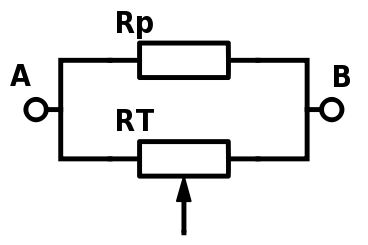
\includegraphics[width=0.75\columnwidth]{parallel.png}
  \caption{
    Parallel circuit
  }
\end{figure}
The expected output $R_{AB}(T)$ for a linearised thermistor setup shown in Fig.\ref{fig:parallel} can be derived from a basic equation for resistor:
\begin{equation}
  \label{eq:Rab}
  R_{AB}(T)=\frac{R_p\cdot R_T(T)}{R_p+R_T(T)}
\end{equation}
\subsection{Time Constant} \label{sub:time}
A time constant, $\tau$ is defined by the time it takes for an element to respond to the change in the surrounding temperature. For example, in this lab experiment, the time constant will define how long it will take for the thermistor to respond to the change from ambient room temperature, to the temperature of iced water. The method of determining the time constant is as follows.

First, the difference between the voltage at ambient room temperature, $V_A$ and the final voltage, $V_O$ in iced water must be found:
$$V_D=V_O-V_A$$
Then, based on the equation
$$f(t)=1-exp(-t)=0.63,\ t=1$$
from Page 59 of J.P. Bentley's Principles and Measurement Systems, this shows that when $\frac{t}{\tau}$ is equal to 1, i.e. one time constant has passed, that 63\% of the total change that will occur due to the new temperature will have happened after $\tau$ has passed. So, multiplying $V_D$ by 0.63 will determine the voltage that will change after one time constant has occurred, $V_\tau$:
$$V_\tau=V_D\times0.63$$
From knowing this value, it is then only necessary to observe the time it takes for the voltage across the thermistor to reach this value from the moment it is submerged into the iced water in order to be able to determine the time constant. Ideally, the system will act in such a way that with each passing time constant, the voltage across the thermistor will increase in relation to the exponential equation listed above, and by 5$\tau$, 99\% of the change will have occurred.
\section{Experiments}
For this lab assignment, two experiments were conducted. The first was to determine the following characteristics of the non-linear response of the NTC:\@ the resistance-temperature R-T and temperature-resistance T-R, the maximum non-linearity $\hat N$ as \% of $f.s.d$ (full scale deflection), and the response of the system linearised by a parallel resistor. The second experiment was done to find the time constant $\tau$ of the measurement system. Raw data from all measurements are presented in the Appendix.

Both of these experiments followed the same basic steps, where the thermistor was placed in an environment with a temperature significantly different from the ambient room temperature --- in a cup filled with either boiling or iced water. The temperature of the environment was measured with a Fluke Thermocouple.
\subsection{R-T and T-R Characteristics}
To measure the R-T and T-R characteristics, the resistance of the thermistor was measured with an AMPROBE AM-510-EUR multimeter, and recorded over a temperature range of 90--45$^{\circ}C$. This was achieved by measuring the temperature of boiling water in a cup, which was cooled from$~100^{\circ}$ to$~45^{\circ}$. As the temperature and the resistance were constantly changing, it was decided to record the setup in video format, in order to collect the necessary data points accurately when some significant temperature change has occurred, for example, every drop of 5 degrees. Having collected this data, the non-linearity of the system can be determined.

Next, a parallel resistor was placed in the system, and the same procedure as previous was followed. In order to establish the necessary value of the parallel resistor, $R_{T_{ctr}}$ was recorded at $T_{ctr}=72.5^{\circ}C$ (the midpoint of the temperature range in which the resistance was measured) and calculated using equation \ref{eq:siemens}, which can also be found in the Siemens handout. Ideally, placing a parallel resistor in the system would help to linearise the change in resistance of the thermistor as a result of the change in temperature of the environment.

As the R-T and T-R characteristics of the thermistor rely on its resistance, it was decided to measure the resistance from the multimeter directly, rather than measure the voltage across as is done in the next experiment.
\subsection{Time Constant}
In order to determine the time constant, the thermistor was again subjected to change in environment temperature, however this time the it was placed in iced water. The iced water throughout this experiment remained at a temperature between$~2^{\circ}$ and$~3^{\circ}$, which was as close to the triple point of water as the conditions would allow. This time, a 2k$\Omega$\ resistor was placed in parallel with the thermistor, and, with the same multimeter, the voltage across the thermistor was measured. This process was recorded again by video, and this was done in order to accurately record the near-exact time it took for the voltage across the thermistor to go from the value at ambient room temperature, to the voltage at the first time constant. It was decided to measure the voltage across the thermistor in this part of the lab assignment, rather than the resistance itself, because the multimeter used in this experiment had a better accuracy for voltage (0.8\% Rdg) than it does for resistance (1.0\% Rdg). As the time constant simply relies on the change in the system over time, and since the voltage across the thermistor is anyway proportional to its resistance, it was decided that the higher accuracy of the voltage reading would lead to a better understanding of the time constant of the thermistor.

This was done three times in order to collect an average on the operational time constant, i.e. the time constant of the thermistor during prolonged use.
\section{Results}
Here, the data from each part the experiments are analysed and discussed. Important graphs, equations, and tables are shown directly in these subsections. Complete calculated data will be put into tables, graphs that can be seen in the Appendix.
\subsection{R-T Characteristics}
\subsubsection{Non-Linear}
The equation for the ideal straight line for input range 45--90$^\circ$ was found using the equation from the datasheet
$$K=\frac{R_T(90)-R_T(45)}{90-45}=\frac{0.915443-4.37181}{90-45}=-0.07681$$aprox
$$a=R_T(45)-KI_{min}=4.37181+0.07681\cdot45=7.828$$
The R-T expected output with combined data from all non-linear measurement runs is shown in the following figure:
\begin{figure}[H]
  \centering
  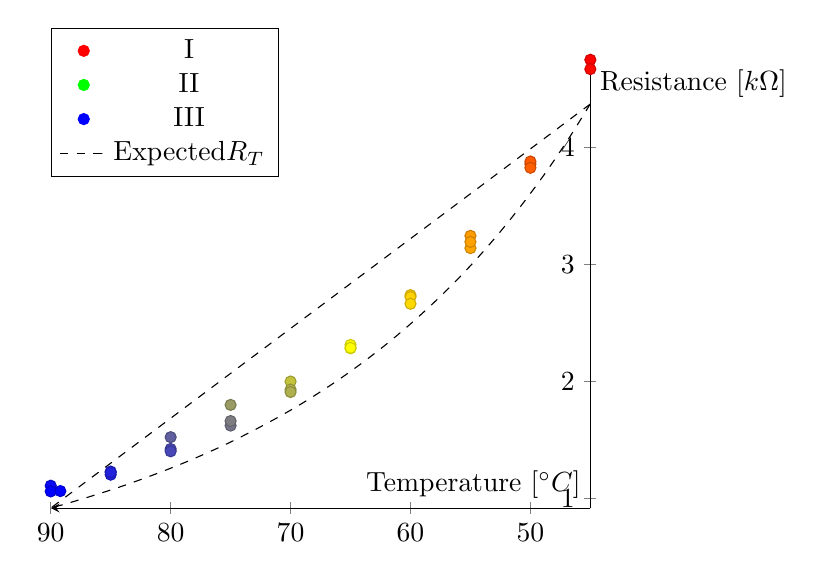
\begin{tikzpicture}
    \begin{axis}[
      axis lines=middle,
      x dir=reverse,
      legend style={
        at={(axis cs:90,3.75)},
        anchor=south west},
      xlabel=Temperature \lbrack$^{\circ}C$\rbrack,
      ylabel=Resistance \lbrack$k\Omega$\rbrack,
      ]
      \addplot[scatter,
      only marks,
      color=red,
      mark=*
      ] coordinates {
        (90, 1.107)
        (85, 1.228)
        (80, 1.522)
        (75, 1.798)
        (70, 1.998)
        (65, 2.311)
        (60, 2.737)
        (55, 3.244)
        (50, 3.858)
        (45, 4.75)
      };
      \addlegendentry{\rom{1}}
      \addplot[scatter,
      only marks,
      color=green,
      mark=*,
      ] coordinates {
        (90, 1.058)
        (85, 1.201)
        (80, 1.421)
        (75, 1.621)
        (70, 1.929)
        (65, 2.282)
        (60, 2.721)
        (55, 3.139)
        (50, 3.88)
        (45, 4.67)
      };
      \addlegendentry{\rom{2}}
      \addplot[scatter,
      only marks,
      color=blue,
      mark=*,
      ] coordinates {
        (89.2, 1.061)
        (85, 1.221)
        (80, 1.401)
        (75, 1.66)
        (70, 1.908)
        (65, 2.286)
        (60, 2.663)
        (55, 3.192)
        (50, 3.826)
      };
      \addlegendentry{\rom{3}}
      \addplot[smooth, black, dashed][domain=45:90]{10*exp(-14.6337+(4791.842/(x+273.15)+(-115334/((x+273.15)^2))+((-3.730535*1000000)/((x+273.15)^3)))};
      \addlegendentry{Expected$R_T$}
      \addplot[smooth, black, dashed][domain=45:90]{-0.0768081*x+7.8281};

    \end{axis}
  \end{tikzpicture}
  \label{fig:without}
  Fig.\ref{fig:without} Non-Linear R-T 
\end{figure}
From the Fig.\ref{fig:without} it can be seen that the thermistors output is non-linear, and the curve shape is similar to the expected response. However, a static offset can be observed, which will be discussed the Error Discussion~\ref{sec:error}.

The T-R characteristic is shown:
\subsubsection{Linear}
Using the eqation~\ref{eq:linear} $R_{p}$ was calculated for linear range 45--90$^{\circ}C$. $B$ value is give in $^{\circ}K$ in the datasheet, but temperature range and measurements are in $^{\circ}C$, therefore it must be converted to Celsius:
$B_C=B_K+273.15=3977-273.15=3703.85$
$$T_{ctr}=\frac{90-45}{2}+45=72.5^{\circ}C$$
$$R_p=1807\cdot\frac{3703.85-72.5}{3703.85+2\cdot72.5}=1.705k\Omega$$
The R-T expected output with combined data from all linear measurement runs is shown in the following figure:
\begin{figure}[H]
  \centering
  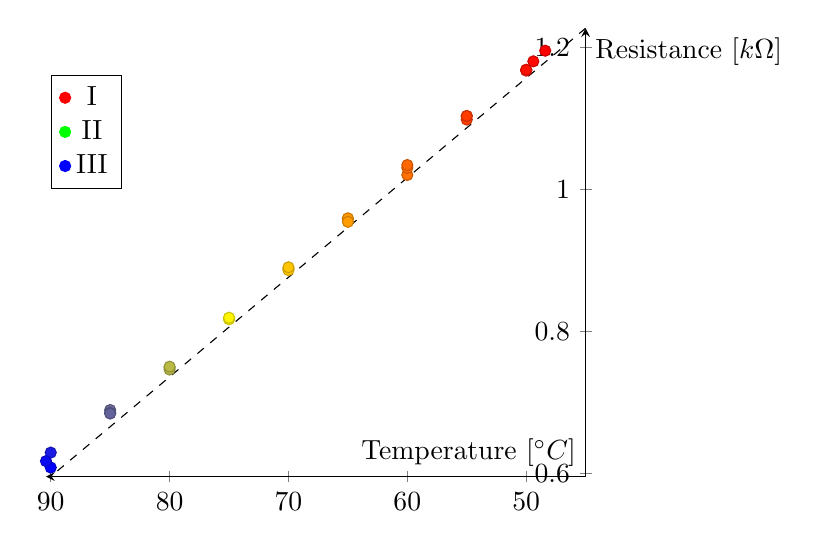
\begin{tikzpicture}
    \begin{axis}[
      axis lines=middle,
      x dir=reverse,
      legend style={
        at={(axis cs:90,1)},
        anchor=south west},
      xlabel=Temperature \lbrack$^{\circ}C$\rbrack,
      ylabel=Resistance \lbrack$k\Omega$\rbrack,
      ]
      \addplot[scatter,
      only marks,
      color=red,
      mark=*,
      ] coordinates {
        (90, 0.608)
        (85, 0.689)
        (80, 0.749)
        (75, 0.817)
        (70, 0.888)
        (65, 0.958)
        (60, 1.02)
        (55, 1.098)
        (50, 1.167)
      };
      \addlegendentry{\rom{1}}
      \addplot[scatter,
      only marks,
      color=green,
      mark=*,
      ] coordinates {
        (90, 0.629)
        (85, 0.685)
        (80, 0.746)
        (75, 0.817)
        (70, 0.886)
        (65, 0.959)
        (60, 1.03)
        (55, 1.103)
        (50, 1.168)
        (48.4, 1.195)
      };
      \addlegendentry{\rom{2}}
      \addplot[scatter,
      only marks,
      color=blue,
      mark=*,
      ] coordinates {
        (90.4, 0.617)
        (85, 0.684)
        (80, 0.75)
        (75, 0.819)
        (70, 0.89)
        (65, 0.954)
        (60, 1.034)
        (55, 1.103)
        (50, 1.168)
        (49.4, 1.18)
      };
      \addlegendentry{\rom{3}}
      \addplot[smooth, black, dashed][domain=45:90]{-0.01403*x+1.858};
    \end{axis}
  \end{tikzpicture}
  \label{fig:with}
  Fig.\ref{fig:with} Linear R-T 
\end{figure}
\subsection{Time Constant}
In order to find the time constant, the voltage across the thermistor was noted at ambient room temperature, $V_A$, and after it has seemingly stabilised in the ice water, $V_O$. Here, these data are shown for the three runs in this part of the lab assignment:
\begin{center}
	\begin{tabular}{c|c|c}
		Run & $V_A$ & $V_O$ \\
		\hline
		\rom{1} & 2.095 & 2.204 \\
		\rom{2} & 2.096 & 2.205 \\
		\rom{3} & 2.098 & 2.201 \\
	\end{tabular}
\end{center}
The calculation for the time constant of Run \rom{1} will be demonstrated here, following that which is mentioned in Section \ref{sub:time}. First, the difference between $V_A$ and $V_O$ is taken to give $V_D$:
$$V_D=2.205-2.095$$
$$V_D=0.11$$
Then, considering that the first time constant, $\tau$ happens at the time at which the change in temperature has reached 63\% of $V_D$,
$$V_\tau=0.108\times0.63$$
$$V_\tau=0.068$$
making $V_t$ to be
$$V_t=2.095+0.068$$
$$V_t=2.164$$
the time constant can then be found by determining the change in time for the voltage across the thermistor to reach $V_t$ from the moment the thermistor had been submerged in the iced water. From the video, this time needs to be estimated, as the value on the multimeter jumps over the desired voltage reading. From estimation (by taking the average time between the voltage read above and below the desired value), the time constant for the first run is 1.382s.

Here, a table is shown with the time constants of the three runs:
\begin{center}
	\begin{tabular}{c|c}
		Run & $\tau$, s \\
		\hline
		\rom{1} & 1.382 \\
		\rom{2} & 1.91 \\
		\rom{3} & 1.498 \\
	\end{tabular}
\end{center}
and here, a table with the expected time, $t_E$, to reach $V_O$ compared to the actual time, $t_A$:
\begin{center}
	\begin{tabular}{c|c|c}
		Run & $t_E$, s & $t_A$, s \\
		\hline
		\rom{1} & 6.91 & 6.025 \\
		\rom{2} & 9.55 & 61.809 \\
		\rom{3} & 7.49 & 6.358 \\
	\end{tabular}
\end{center}

An average of the three results have been taken, and put into a graph in Fig. \ref{fig:timeresponseresult}.1 in order to analyse the nature of response of the thermistor to that shown on Page 59 of J.P. Bentley's Principles and Measurement Systems, modified in Fig. \ref{fig:timeresponseideal}.2. It can be seen that in the average time response function of the thermistor, it appears to approach the average $V_O$, however when compared to the expected time response function, it does not follow this trend.

\begin{figure}[H]
	\centering
	\begin{tikzpicture}
	\begin{axis}[
	axis lines=middle,
	xlabel=$\tau$ \lbrack s\rbrack, ylabel=Voltage \lbrack V\rbrack]
	\addplot[smooth,
	color=black,
	mark=*,
	error bars/.cd,y dir=both,
	y explicit
	] coordinates {
		(1.59667, 2.16395)
		(3.19333, 2.18971)
		(4.79, 2.1983)
		(6.38667, 2.20152)
		(7.98333, 2.20259)
	};
	\addplot[draw=red, dashed][domain=0:8]{2.20367};
	\end{axis}
	\end{tikzpicture}
	\label{fig:timeresponseresult}
	Figure 4.2.1: Time Response Function of Thermistor Compared to Average $V_O$
\end{figure}

\begin{figure}[H]
	\centering
	\begin{tikzpicture}
	\begin{axis}[
	axis lines=middle,
	xlabel=$\tau$ \lbrack s\rbrack, ylabel=Voltage \lbrack V\rbrack]
	\addplot[smooth,
	color=black,
	mark=*,
	error bars/.cd,y dir=both,
	y explicit
	] coordinates {
		(1.59667, 2.16395)
		(3.19333, 2.18971)
		(4.79, 2.1983)
		(6.38667, 2.20152)
		(7.98333, 2.20259)
	};
	\addplot[draw=red, dashed][domain={0:8}]{2.20367-2.20367*exp(-x)};
	\end{axis}
	\end{tikzpicture}
	\label{fig:timeresponseideal}
	Figure 4.2.2: Time Response Function of Thermistor Compared to Expected Result
\end{figure}

\section{Error Discussion}
\label{sec:error}
\subsection{Time Constant}
The calculated function including the time constant for this part of the lab assignment appears to tend towards $V_O$, however, this may simply be due to the nature of how the function was calculated. It can be seen that the function does not follow that of the expected outcome, and this may be attributed to the fact that there was no accurate way of gathering the data from the time. As the video was not started the exact moment the thermistor was submerged into the iced water, a guess needed to be made towards when exactly the time measurement should stop. Additionally, as the voltage values assumed to be seen at the time of the first time constant $V_\tau$ were never read by the multimeter, there was more guessing that needed to be done in order to determine the time at which this voltage was reached. Additional error can come from the delay that the multimeter has when displaying the voltage, as it is not capable of displaying the voltage accurately in relation to the time that it is reached. Furthermore, there is some fluctuation in the voltage reading near what is assumed to be $V_O$, and this can mainly be attributed to the temperature of the iced water not being constant, i.e. some parts of the iced water may be colder or warmer than others, and the thermistor moving around in the different temperatures.
\section{Conclusion}
\#stirring cup of ice water
\onecolumn
\begin{thebibliography}{99}
	\bibitem{SAA}
	J.P.\ Bentley, \textit{Principles of Measurement Systems, 4th Edition},
	(Pearson Education Limited, England, 2005).
	
	\bibitem{Datasheet} \emph{AM-510 Digital Multimeter},   available at
	\texttt{http://content.amprobe.com/DataSheets/AM-510
		\%20Digital\%20Multimeter.pdf}.	
\end{thebibliography}
\appendix
\section{Tables}
\begin{table}[H]
	\centering
	\caption{Time Constant: Run \rom{1}}
	\label{const1}
	\begin{tabular}{l|l}
		$\tau$, s  &  Expected Voltage, V \\
		\hline
		1.382 &  2.164 \\
		2.764 &  2.191 \\
		4.146 & 2.196 \\
		5.528 & 2.203 \\
		6.91 & 2.204 \\
	\end{tabular}
\end{table}
\begin{table}[H]
	\centering
	\caption{Time Constant: Run \rom{2}}
	\label{const2}
	\begin{tabular}{l|l}
		$\tau$, s  &  Expected Voltage, V \\
		\hline
		1.91 &  2.164 \\
		3.82 &  2.191 \\
		5.73 & 2.196 \\
		7.64 & 2.203 \\
		9.55 & 2.204 \\
	\end{tabular}
\end{table}
\begin{table}[H]
	\centering
	\caption{Time Constant: Run \rom{3}}
	\label{const3}
	\begin{tabular}{l|l}
		$\tau$, s  &  Expected Voltage, V \\
		\hline
		1.498 &  2.164 \\
		2.996 &  2.190 \\
		4.494 & 2.198 \\
		5.992 & 2.202 \\
		7.49 & 2.203 \\
	\end{tabular}
\end{table}
\section{Graphs}
\end{document}